%! Author = wolfram_e_laube
%! Date = 06.05.24

\item[(b)]
\section{Exercise 1 Task (b): Visualization of Sampling Effects on Spectrum}

\subsection{Problem Statement}
Given a signal with frequency components at 4 kHz and 6 kHz, this task involves visualizing the impact of a 10 kHz sampling frequency on its spectrum. The objective is to illustrate the original spectrum, the spectrum shifted by $-f_s$ and $+f_s$, and the combined result to demonstrate potential overlaps and aliasing effects due to sampling.

\subsection{Objective}
The goal is to:
\begin{itemize}
    \item Show the original spectrum with components at $\pm 4$ kHz and $\pm 6$ kHz.
    \item Illustrate the effects of shifting this spectrum by the sampling frequency ($\pm 10$ kHz).
    \item Display the combined spectrum to identify any aliasing or overlap issues that occur due to these shifts.
\end{itemize}

\subsection{Visualization Method}
The spectral components and their shifts are visualized using Python and Matplotlib, with the following approach:

\begin{verbatim}
# Python code snippet for visualization
import numpy as np
import matplotlib.pyplot as plt

# Frequencies of the original signal
original_frequencies = np.array([-6000, -4000, 4000, 6000])
amplitude = np.array([1, 1, 1, 1])

# Sampling frequency
fs = 10000

# Plotting
plt.figure(figsize=(12, 6))
plt.stem(original_frequencies, amplitude, linefmt='C0-', markerfmt='C0o', basefmt=" ", label='Original Spectrum')
plt.stem(original_frequencies - fs, amplitude * 0.8, linefmt='C1-', markerfmt='C1o', basefmt=" ", label='Shifted Spectrum $-f_s$')
plt.stem(original_frequencies + fs, amplitude * 0.8, linefmt='C2-', markerfmt='C2o', basefmt=" ", label='Shifted Spectrum $+f_s$')
plt.title('Effect of Sampling on Signal Spectrum')
plt.xlabel('Frequency (Hz)')
plt.ylabel('Amplitude')
plt.legend()
plt.grid(True)
plt.show()
\end{verbatim}

\subsection{Conclusion}
The visualization clearly demonstrates that sampling a signal with components near or above half the sampling frequency can lead to significant aliasing. The 6 kHz component, when shifted by the 10 kHz sampling frequency, aliases into the 4 kHz component, reinforcing its amplitude due to overlapping spectral lines. This underscores the critical need for appropriate sampling rates to avoid distortions and ensure accurate digital representation of analog signals.

\begin{figure}[h]
    \centering
    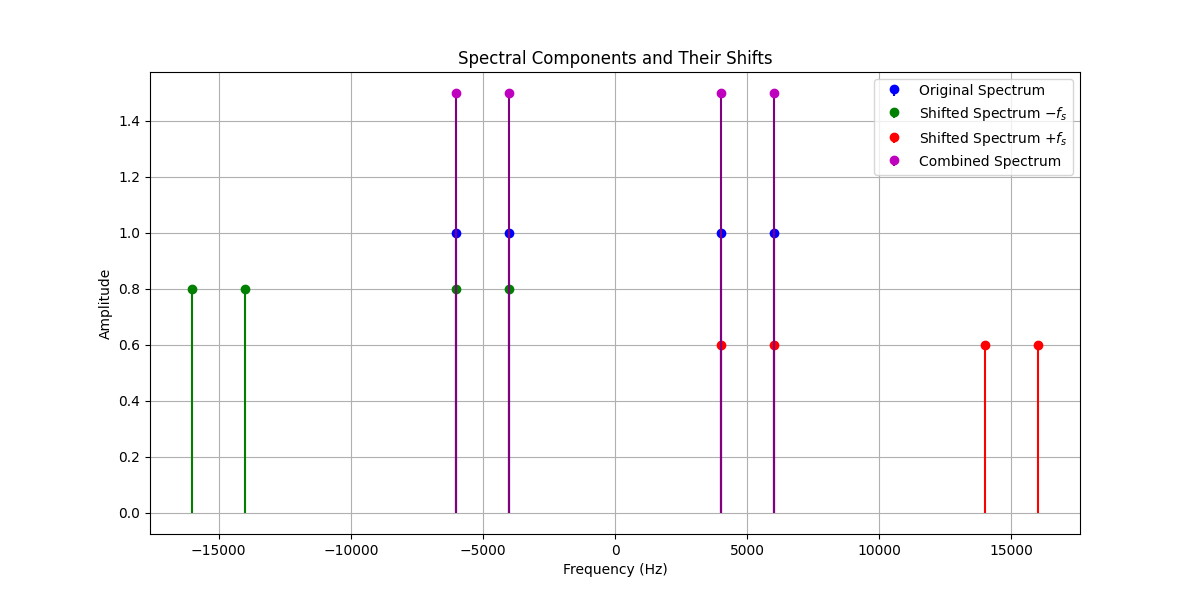
\includegraphics[width=0.49\textwidth]{fig/ex1_b_plot}
    \caption{Spectrum of \(x(t)\)}
    \label{fig:ex1_b_plot}
\end{figure}

The shifted spectrum plot will show the spectral shifts due to the sampling frequency and illustrate the overlapping spectra.